% !TeX spellcheck = en_GB
\section{Integrated Vapour Transport}
 \label{sec:weather:atm_riv}
% An atmospheric river (AR) is a filament structure of intense moisture transport from the tropics to higher latitudes. Heavy precipitation can be associated with it, because the air is warm and moist. This can often be observed at mountain ranges at west coasts such as in Norway \citep{azad_extreme_2017}. Due to orographic lifting the moisture will be released and follow high amounts of precipitation. 
% \\
% An atmospheric river is characterised if the integrated vapour transport shows values higher than \SI{250}{\IVT} and a continuous region larger than \SI{2000}{\km} \citep{rutz_climatological_2014}.
% \\
\Cref{fig:AR24_pres} shows coloured contours of the integrated vapour transport (IVT) in \SI{}{\IVT}, where warmer colours indicate higher IVT. 
Stream vectors in \Cref{fig:AR24_pres} indicate the direction and intensity of the IVT flow. 
% The integrated vapour transport (IVT) was calculated from the ECMWF data as followed:
% \begin{align}
% IVT = \frac{1}{g} \int\limits_{p_{sfc}}^{\SI{100}{\hPa}} q \mathbf{V} dp \qquad [\SI{}{\IVT}]
% \label{eq:IVT}
% \end{align} 
% where $g$ is the standard gravity, $q$ the specific humidity, and $\mathbf{V}$ the total wind vector at each pressure level $p$. The numerical, trapezoidal integration is performed by using data from the surface pressure $p_{sfc}$ to \SI{850}{\hPa} in \SI{50}{\hPa} intervals and from \SIrange{700}{100}{\hPa} in \SI{100}{\hPa} intervals.
\\
Analysing integrated vapour transport maps is important, since extreme precipitation events in Norway are often influenced by moist, warm air advection from the tropics \citep{azad_extreme_2017}. \Cref{fig:AtmRiv} shows integrated vapour transport from the tropics to the midlatitudes, but it also presents that the occurrence of the atmospheric river was not the main factor which led to intense precipitation during the 2016 Christmas storm. 
Since it showed not to be intense it will not be further discussed.
%%% Atmospheric river maps %%%%%%%%%%%%%%%%%%%%%%%%%%%%%%%%%%%%%
\begin{figure}[H]
	\centering
	%%%%%% 20/12
	\begin{subfigure}[b]{0.49\textwidth}
		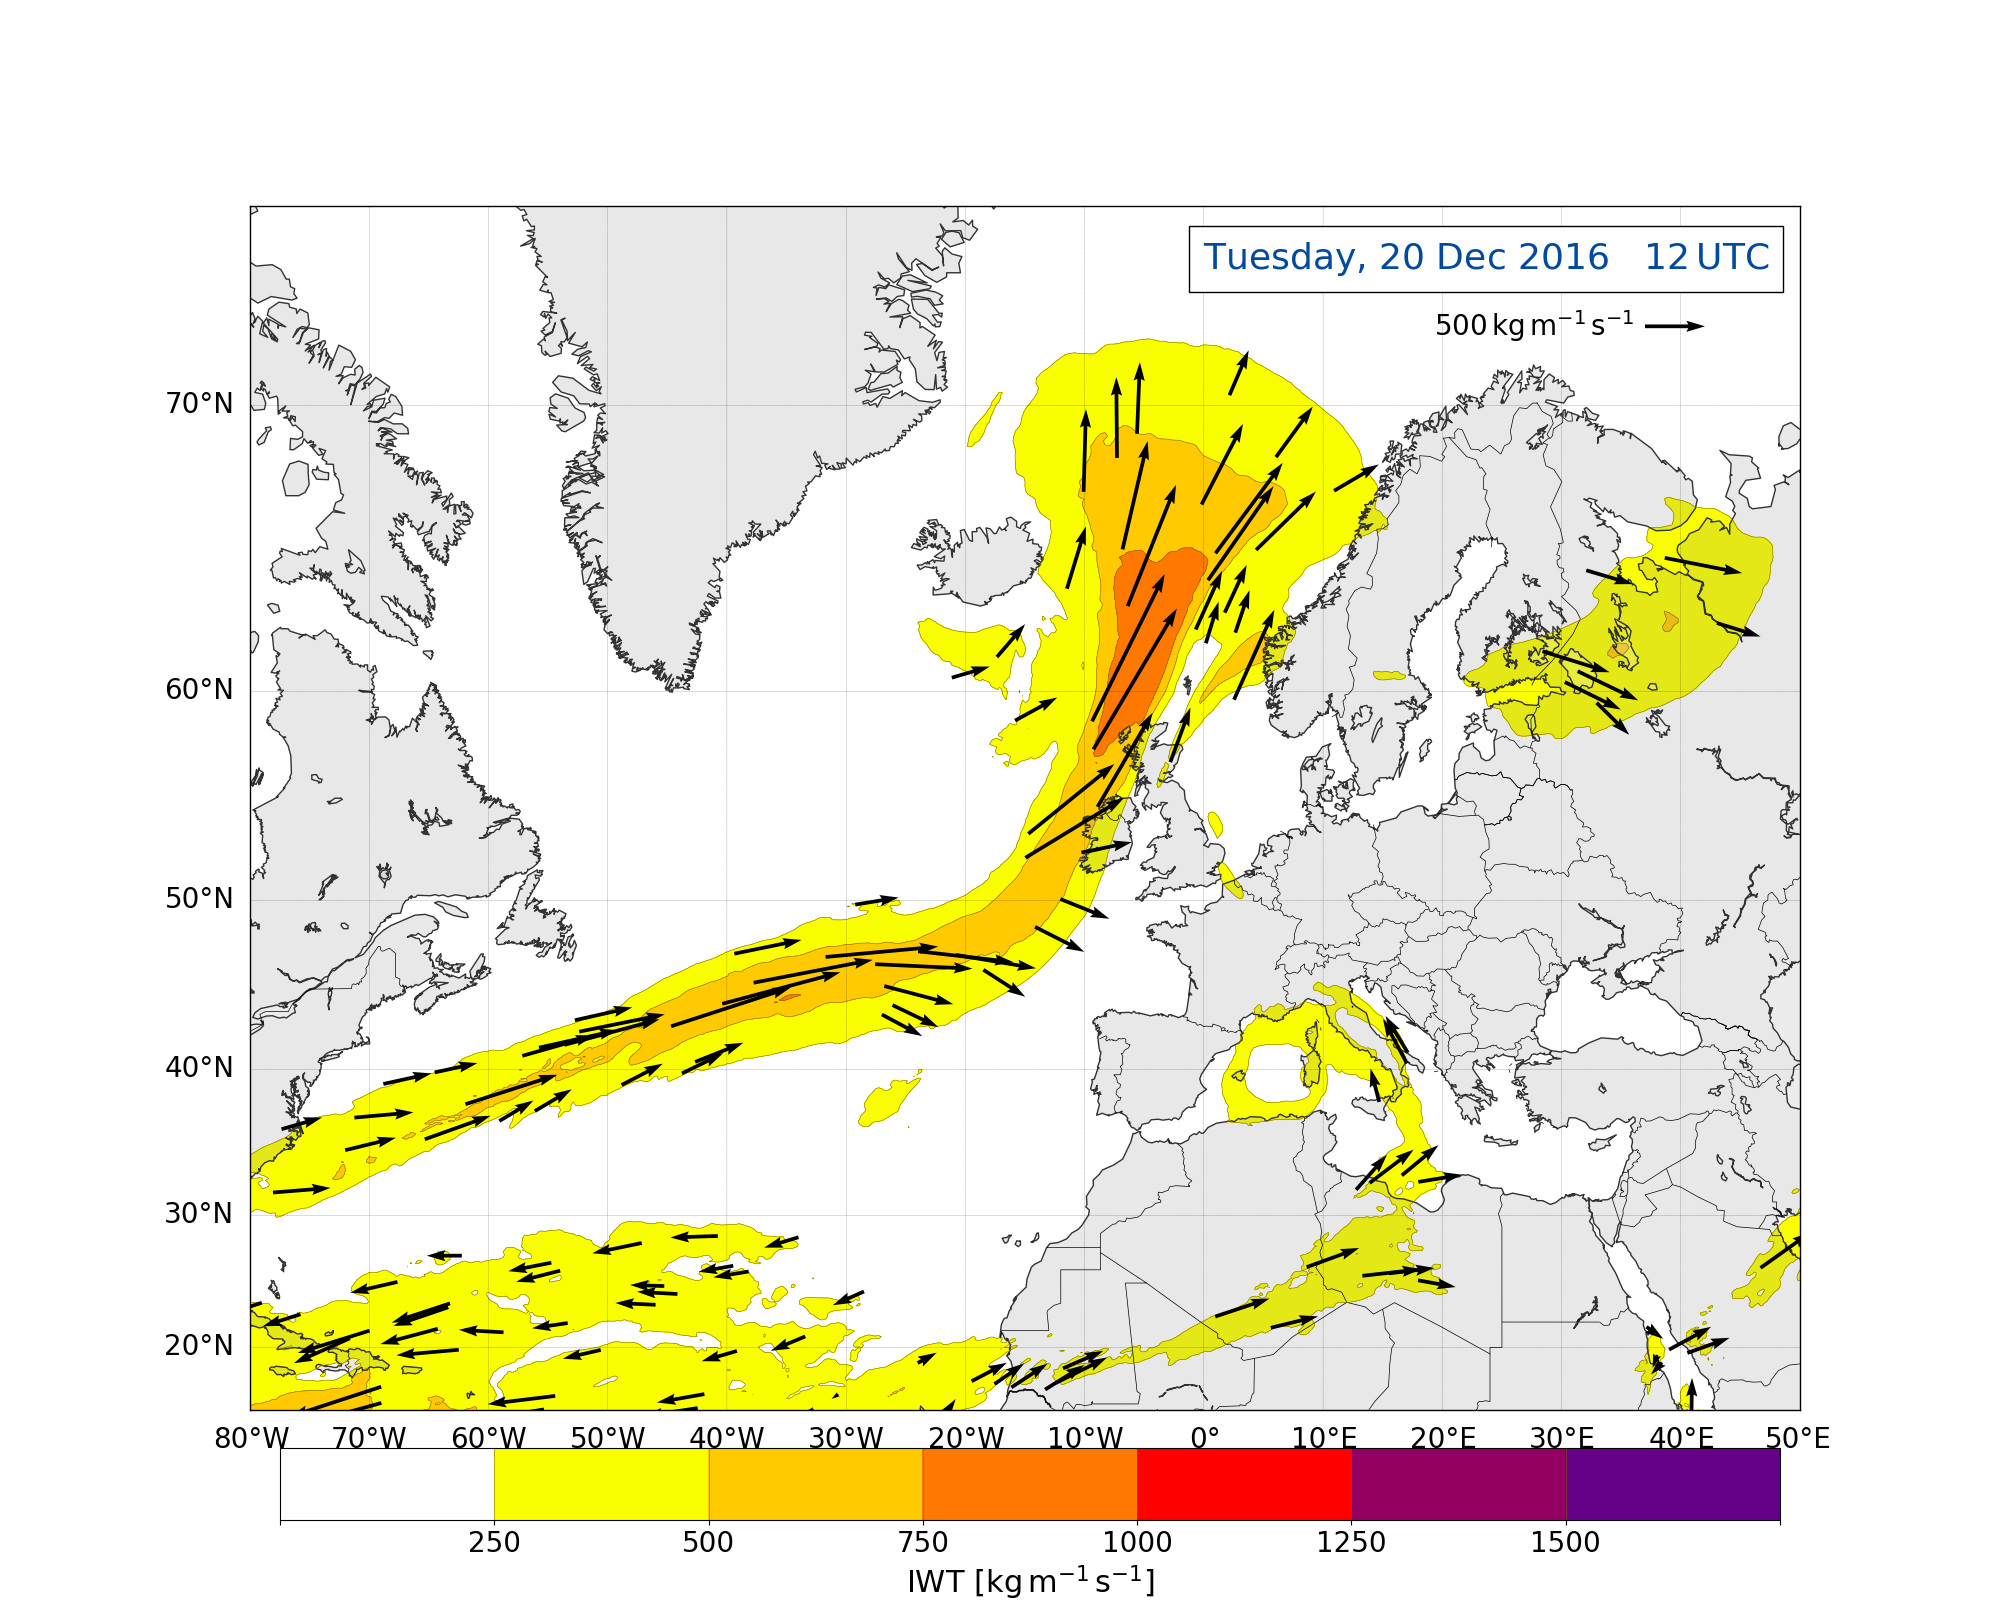
\includegraphics[trim={4.2cm 3.9cm 4.3cm 5.1cm},clip,
		width=\textwidth]{./fig_Atm_Riv/20161220_12}
		\caption{}\label{fig:AR20}
	\end{subfigure}
	%%%%%% 21/12
	\begin{subfigure}[b]{0.49\textwidth}
		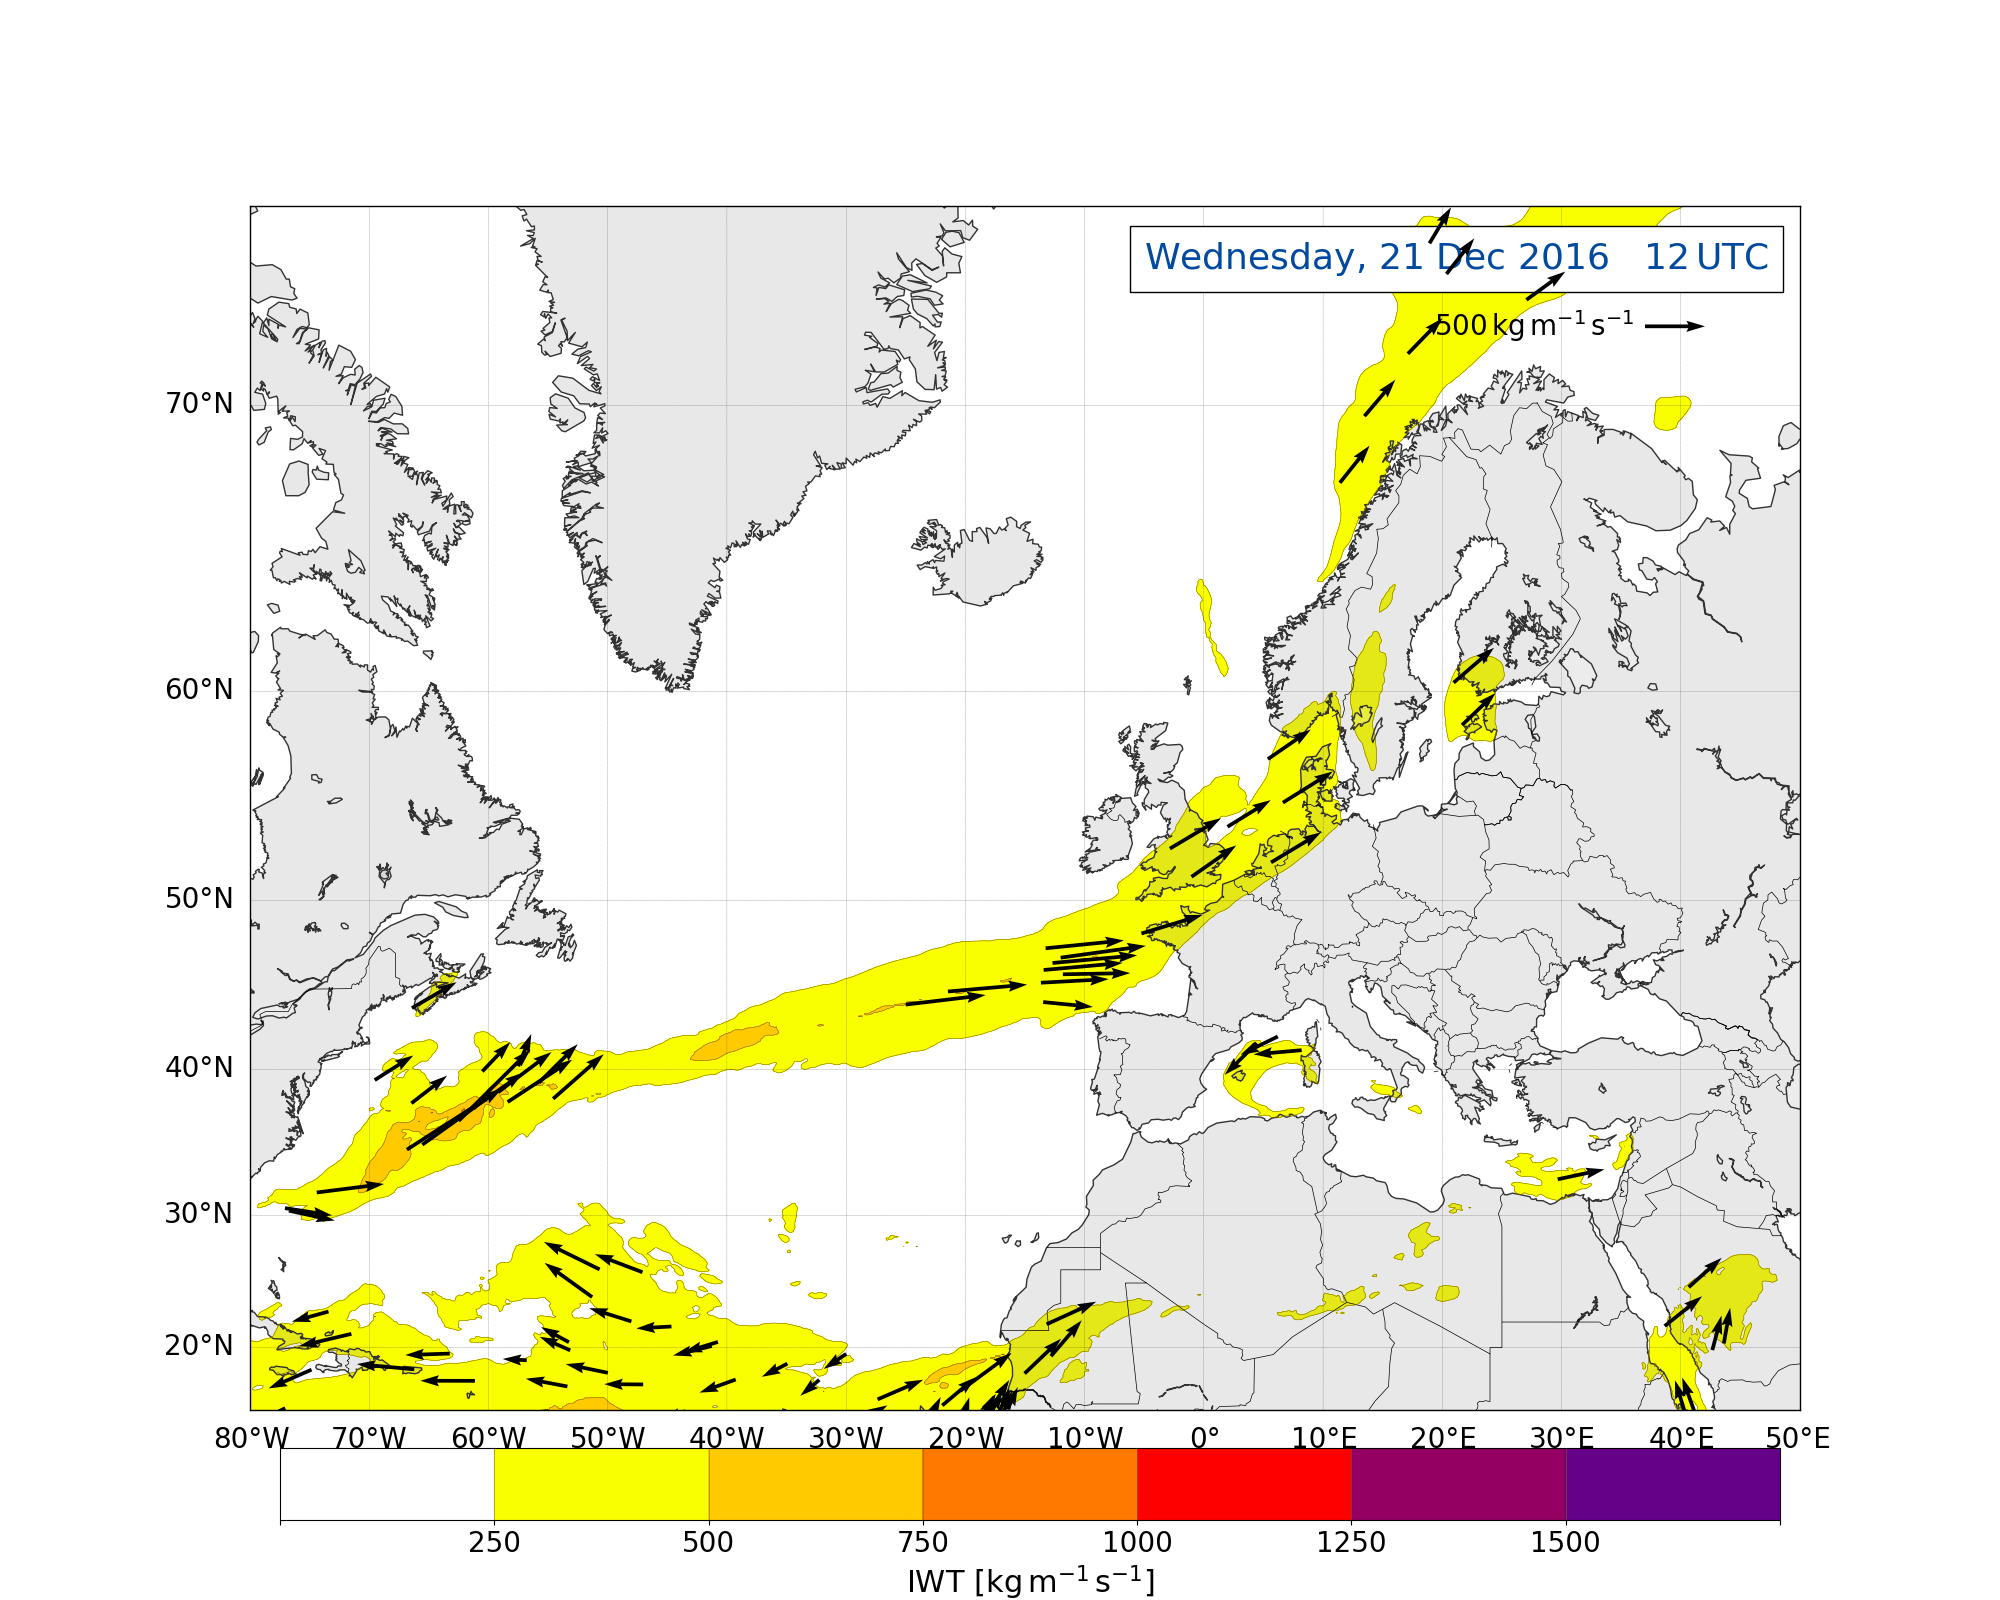
\includegraphics[trim={4.2cm 3.9cm 4.3cm 5.1cm},clip,
		width=\textwidth]{./fig_Atm_Riv/20161221_12}
		\caption{}\label{fig:AR21}
	\end{subfigure}
    %%%%%% 22/12
	\begin{subfigure}[b]{0.49\textwidth}
		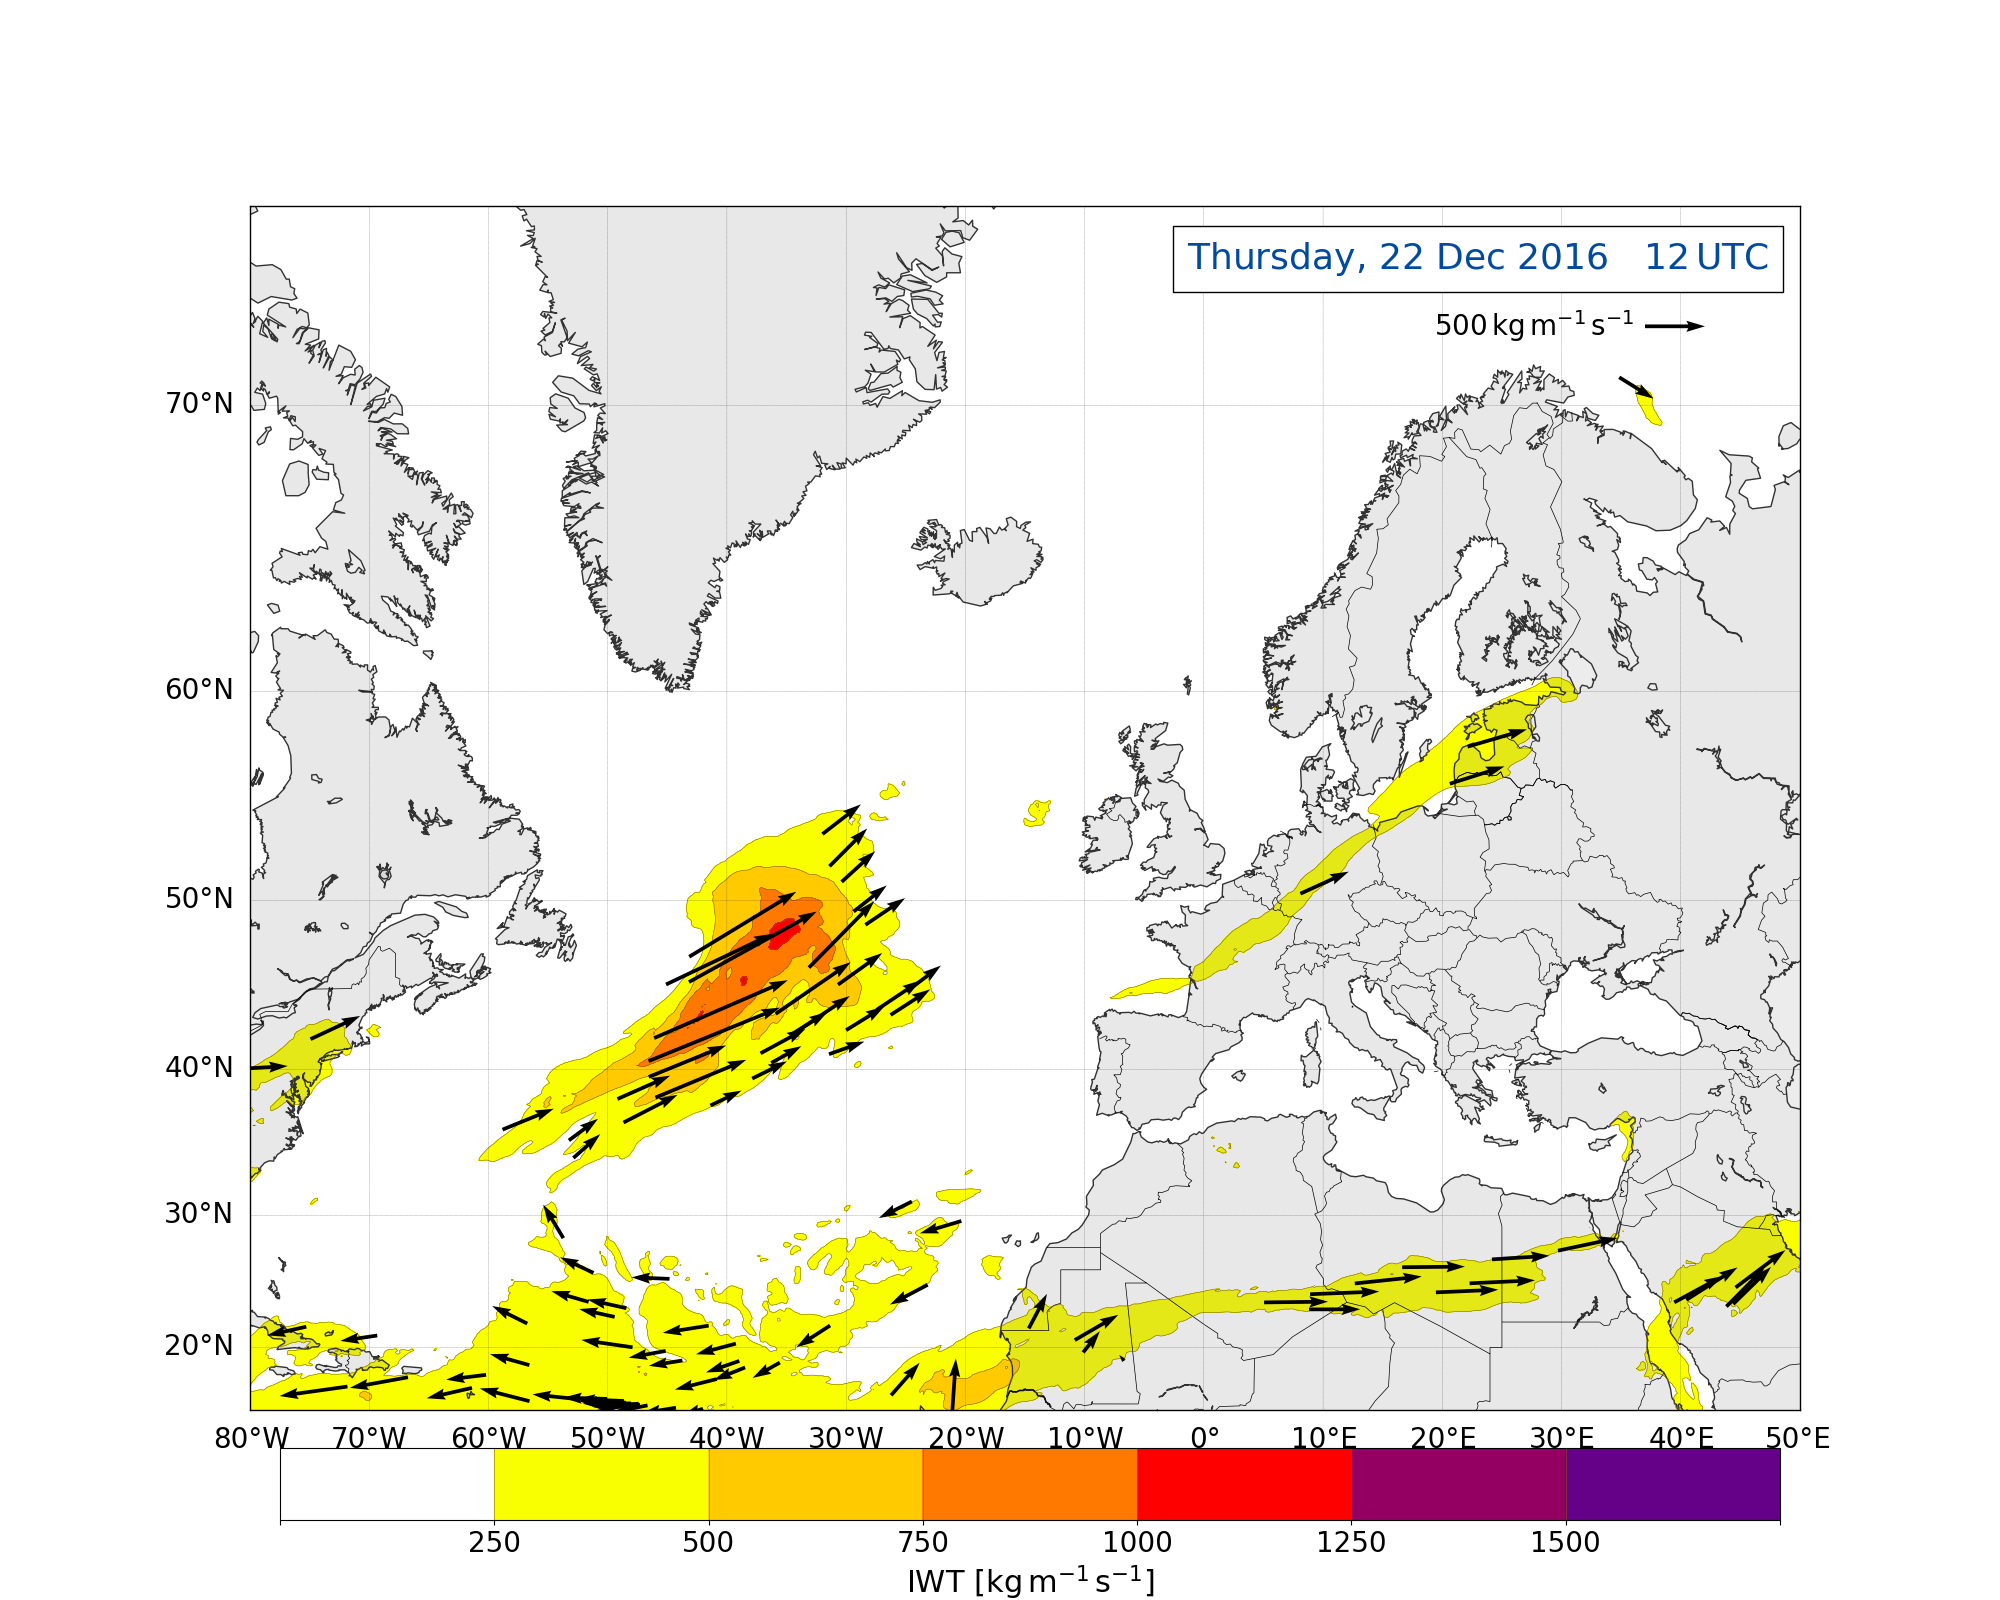
\includegraphics[trim={4.2cm 3.9cm 4.3cm 5.1cm},clip,
		width=\textwidth]{./fig_Atm_Riv/20161222_12}
		\caption{}\label{fig:AR22}
		%\label{fig:sfc2100}
	\end{subfigure}
	%%%%%% 23/12
	\begin{subfigure}[b]{0.49\textwidth}
		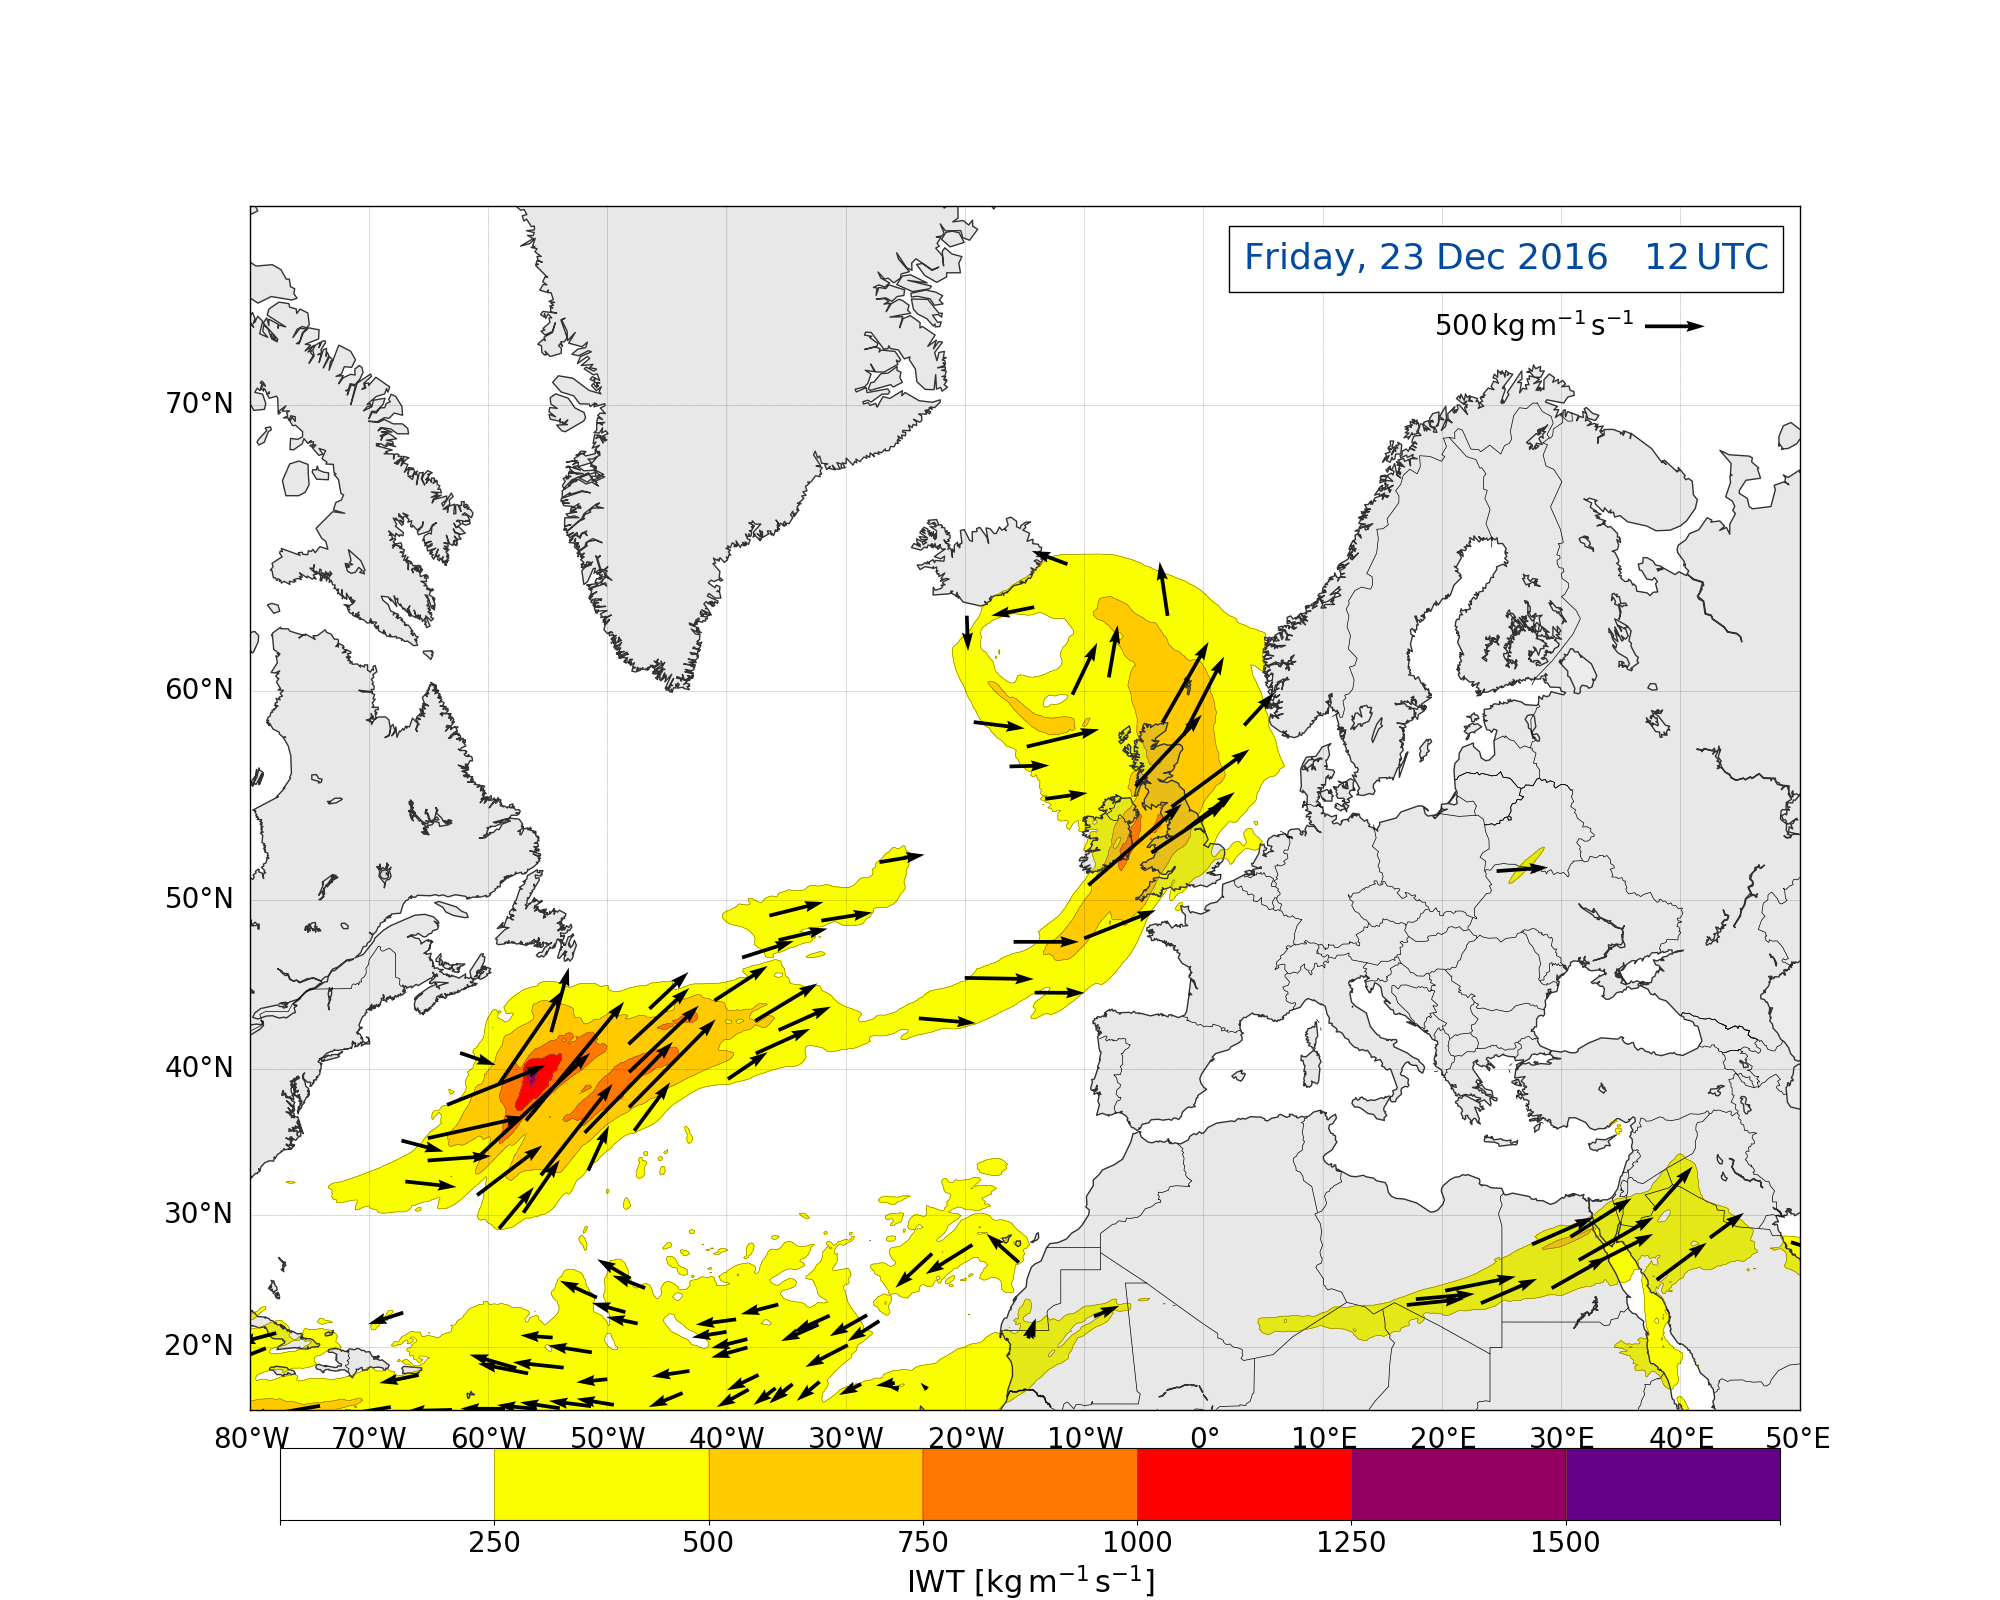
\includegraphics[trim={4.2cm 3.9cm 4.3cm 5.1cm},clip,
		width=\textwidth]{./fig_Atm_Riv/20161223_12}
		\caption{}\label{fig:AR23}
	\end{subfigure}
	%%%%%% label
	\begin{subfigure}[b]{\textwidth}
		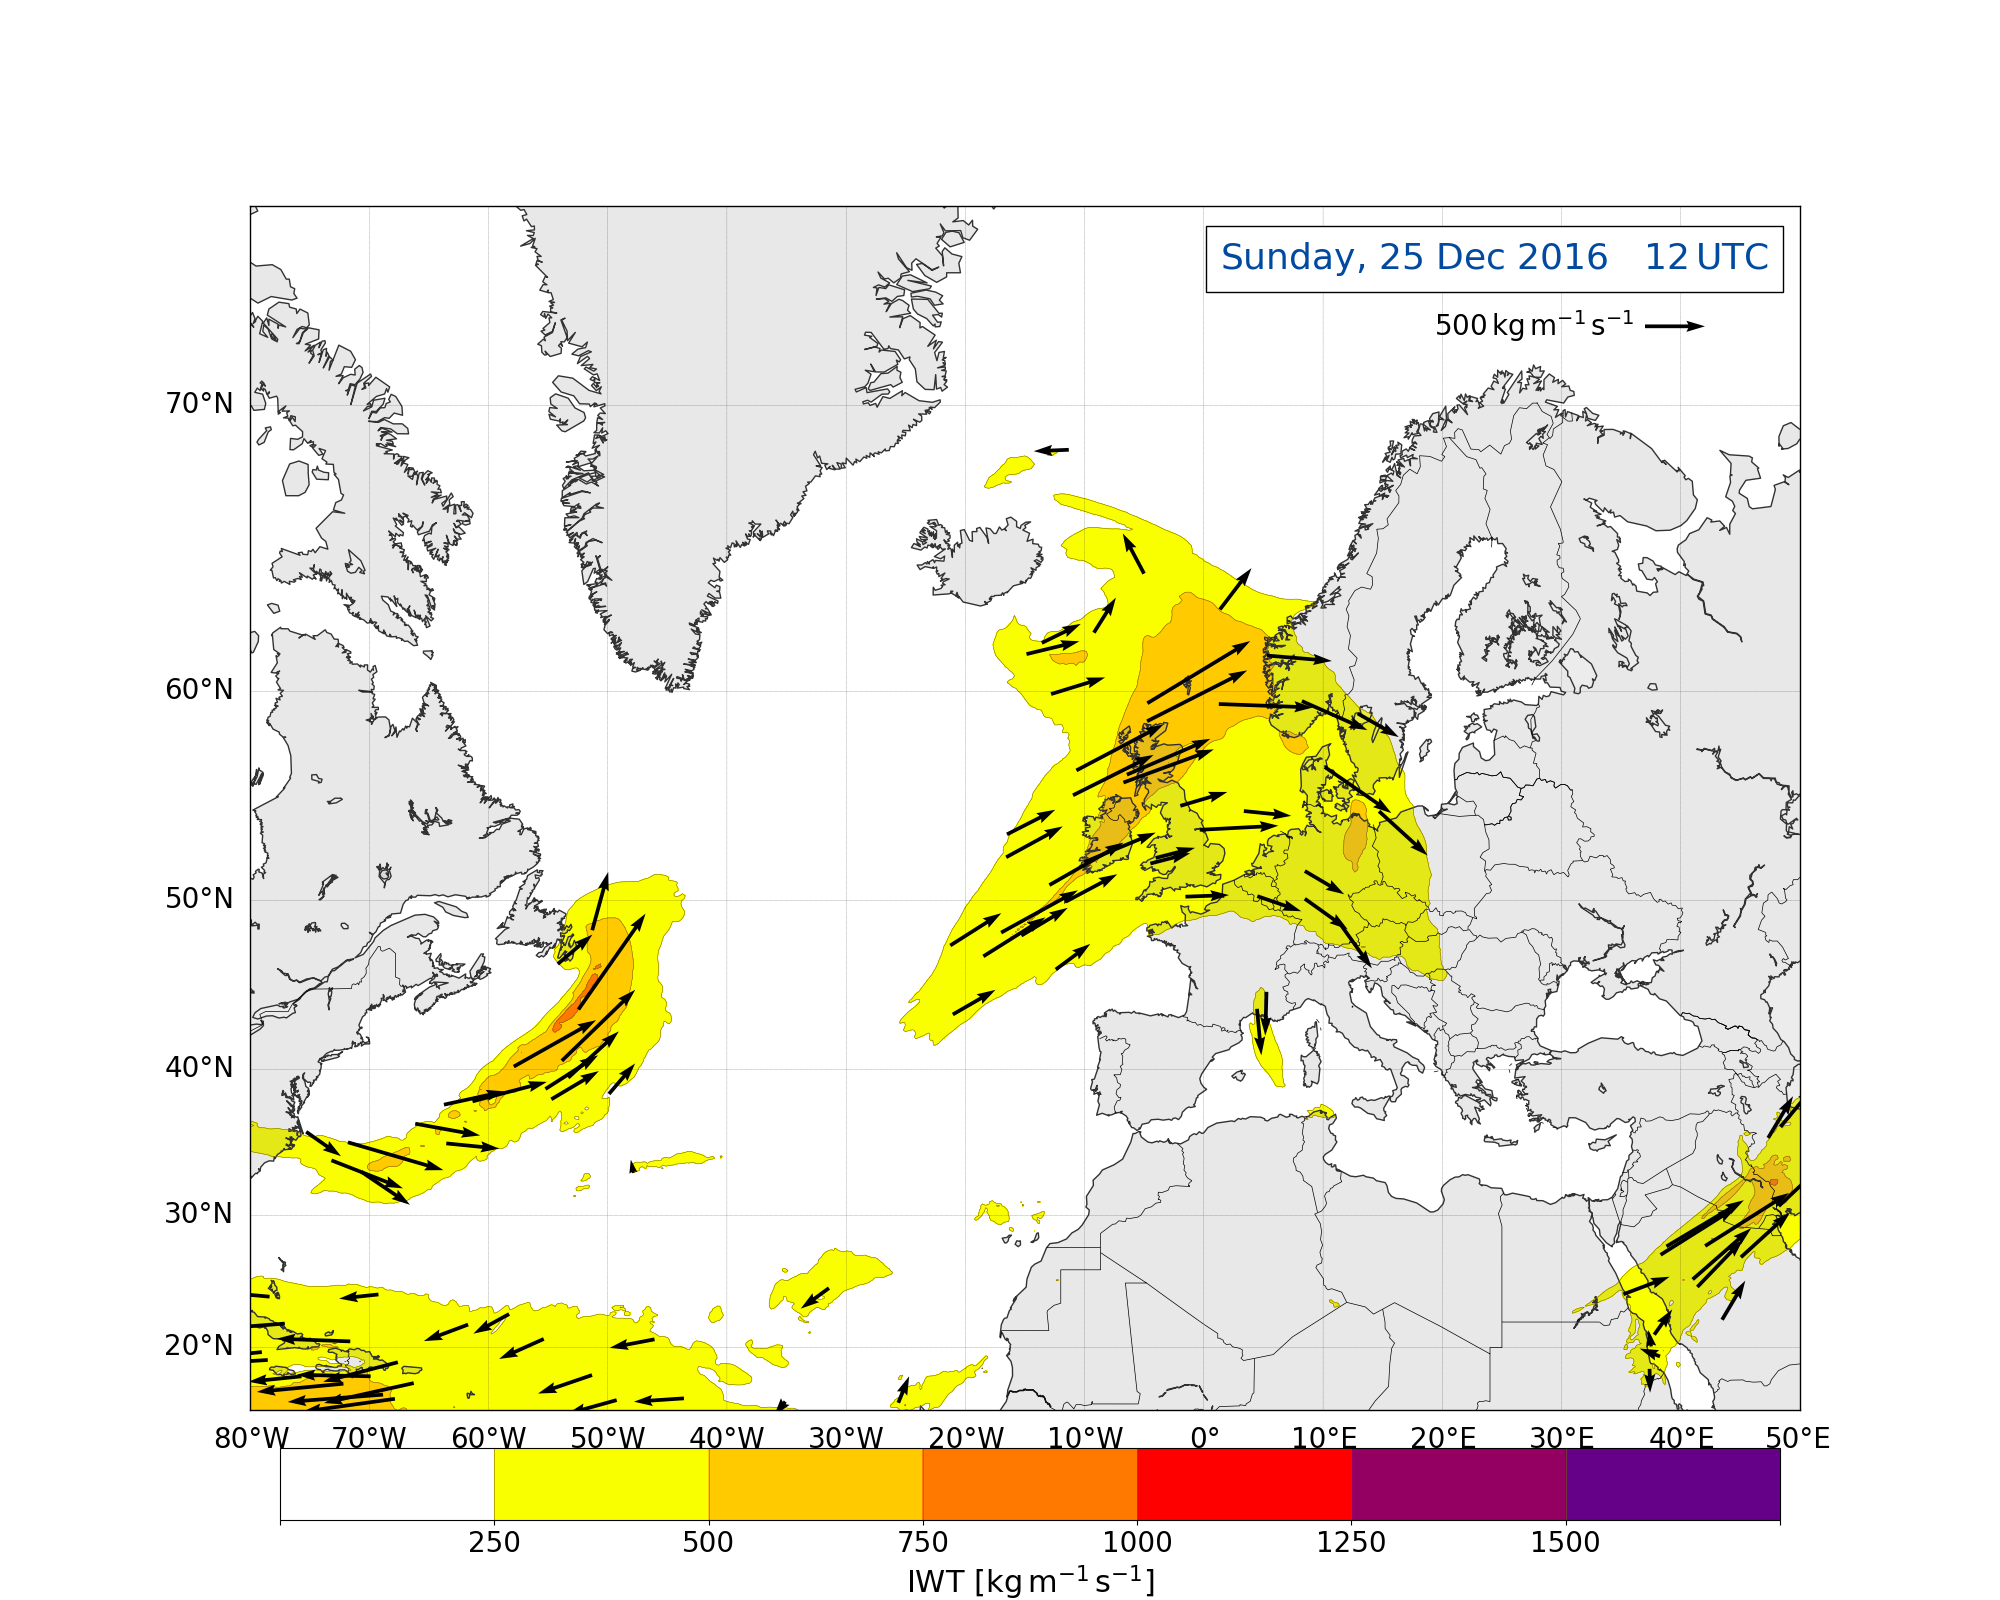
\includegraphics[trim={4.2cm 0cm 4.3cm 36.8cm},clip,
		width=\textwidth]{./fig_Atm_Riv/20161225_12}
	\end{subfigure}
\caption{Atmospheric river analysis map, data from ECMWF. During \SIrange{20}{27}{\dec}. IVT, shaded according to the colour bar [\SI{}{\IVT}]. Vectors, indicating the direction and magnitude of the IVT. }\label{fig:AtmRiv}
\end{figure}
%%%%%%%%%%%%%%%%%%%%%%%%%%%%%%%%%%%%%%%%%%%%%%%%%%%%%%%%%%%%%%%%%%%%%%%%%
\noindent
%% Atmospheric river maps %%%%%%%%%%%%%%%%%%%%%%%%%%%%%%%%%%%%%
\begin{figure}[t!]\ContinuedFloat
	%%%%%% 24/12
	\begin{subfigure}[b]{0.49\textwidth}
		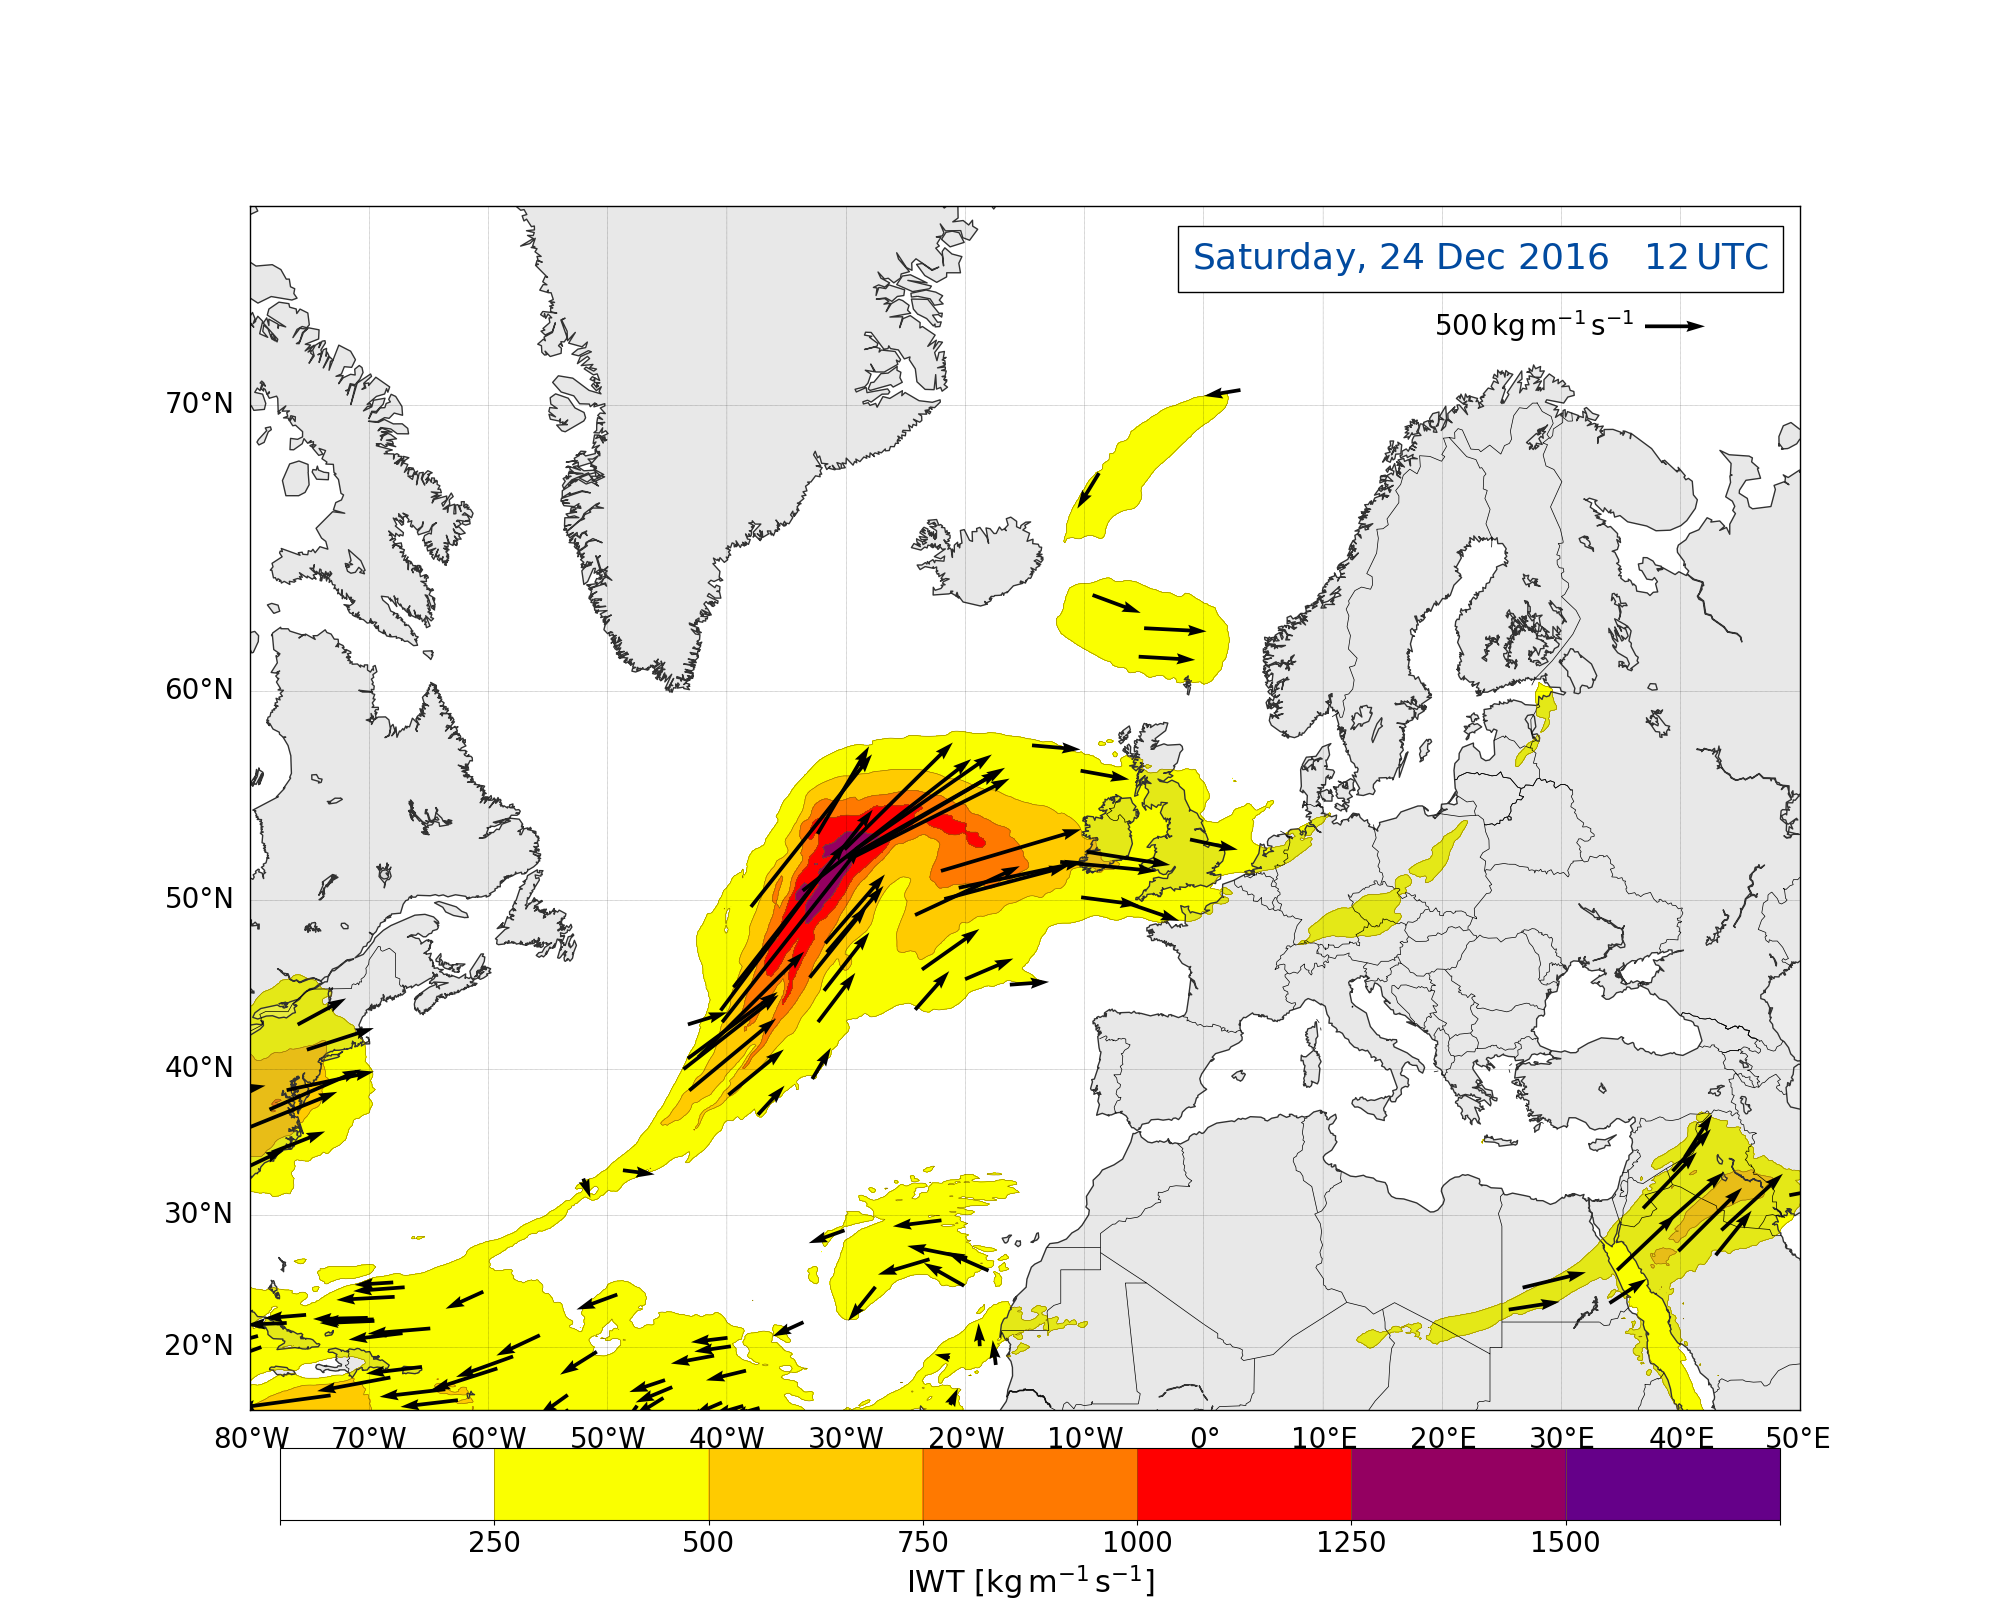
\includegraphics[trim={4.2cm 3.9cm 4.3cm 5.1cm},clip,
		width=\textwidth]{./fig_Atm_Riv/20161224_12}
		\caption{}\label{fig:AR24}
	\end{subfigure}
	%%%%%% 25/12
	\begin{subfigure}[b]{0.49\textwidth}
		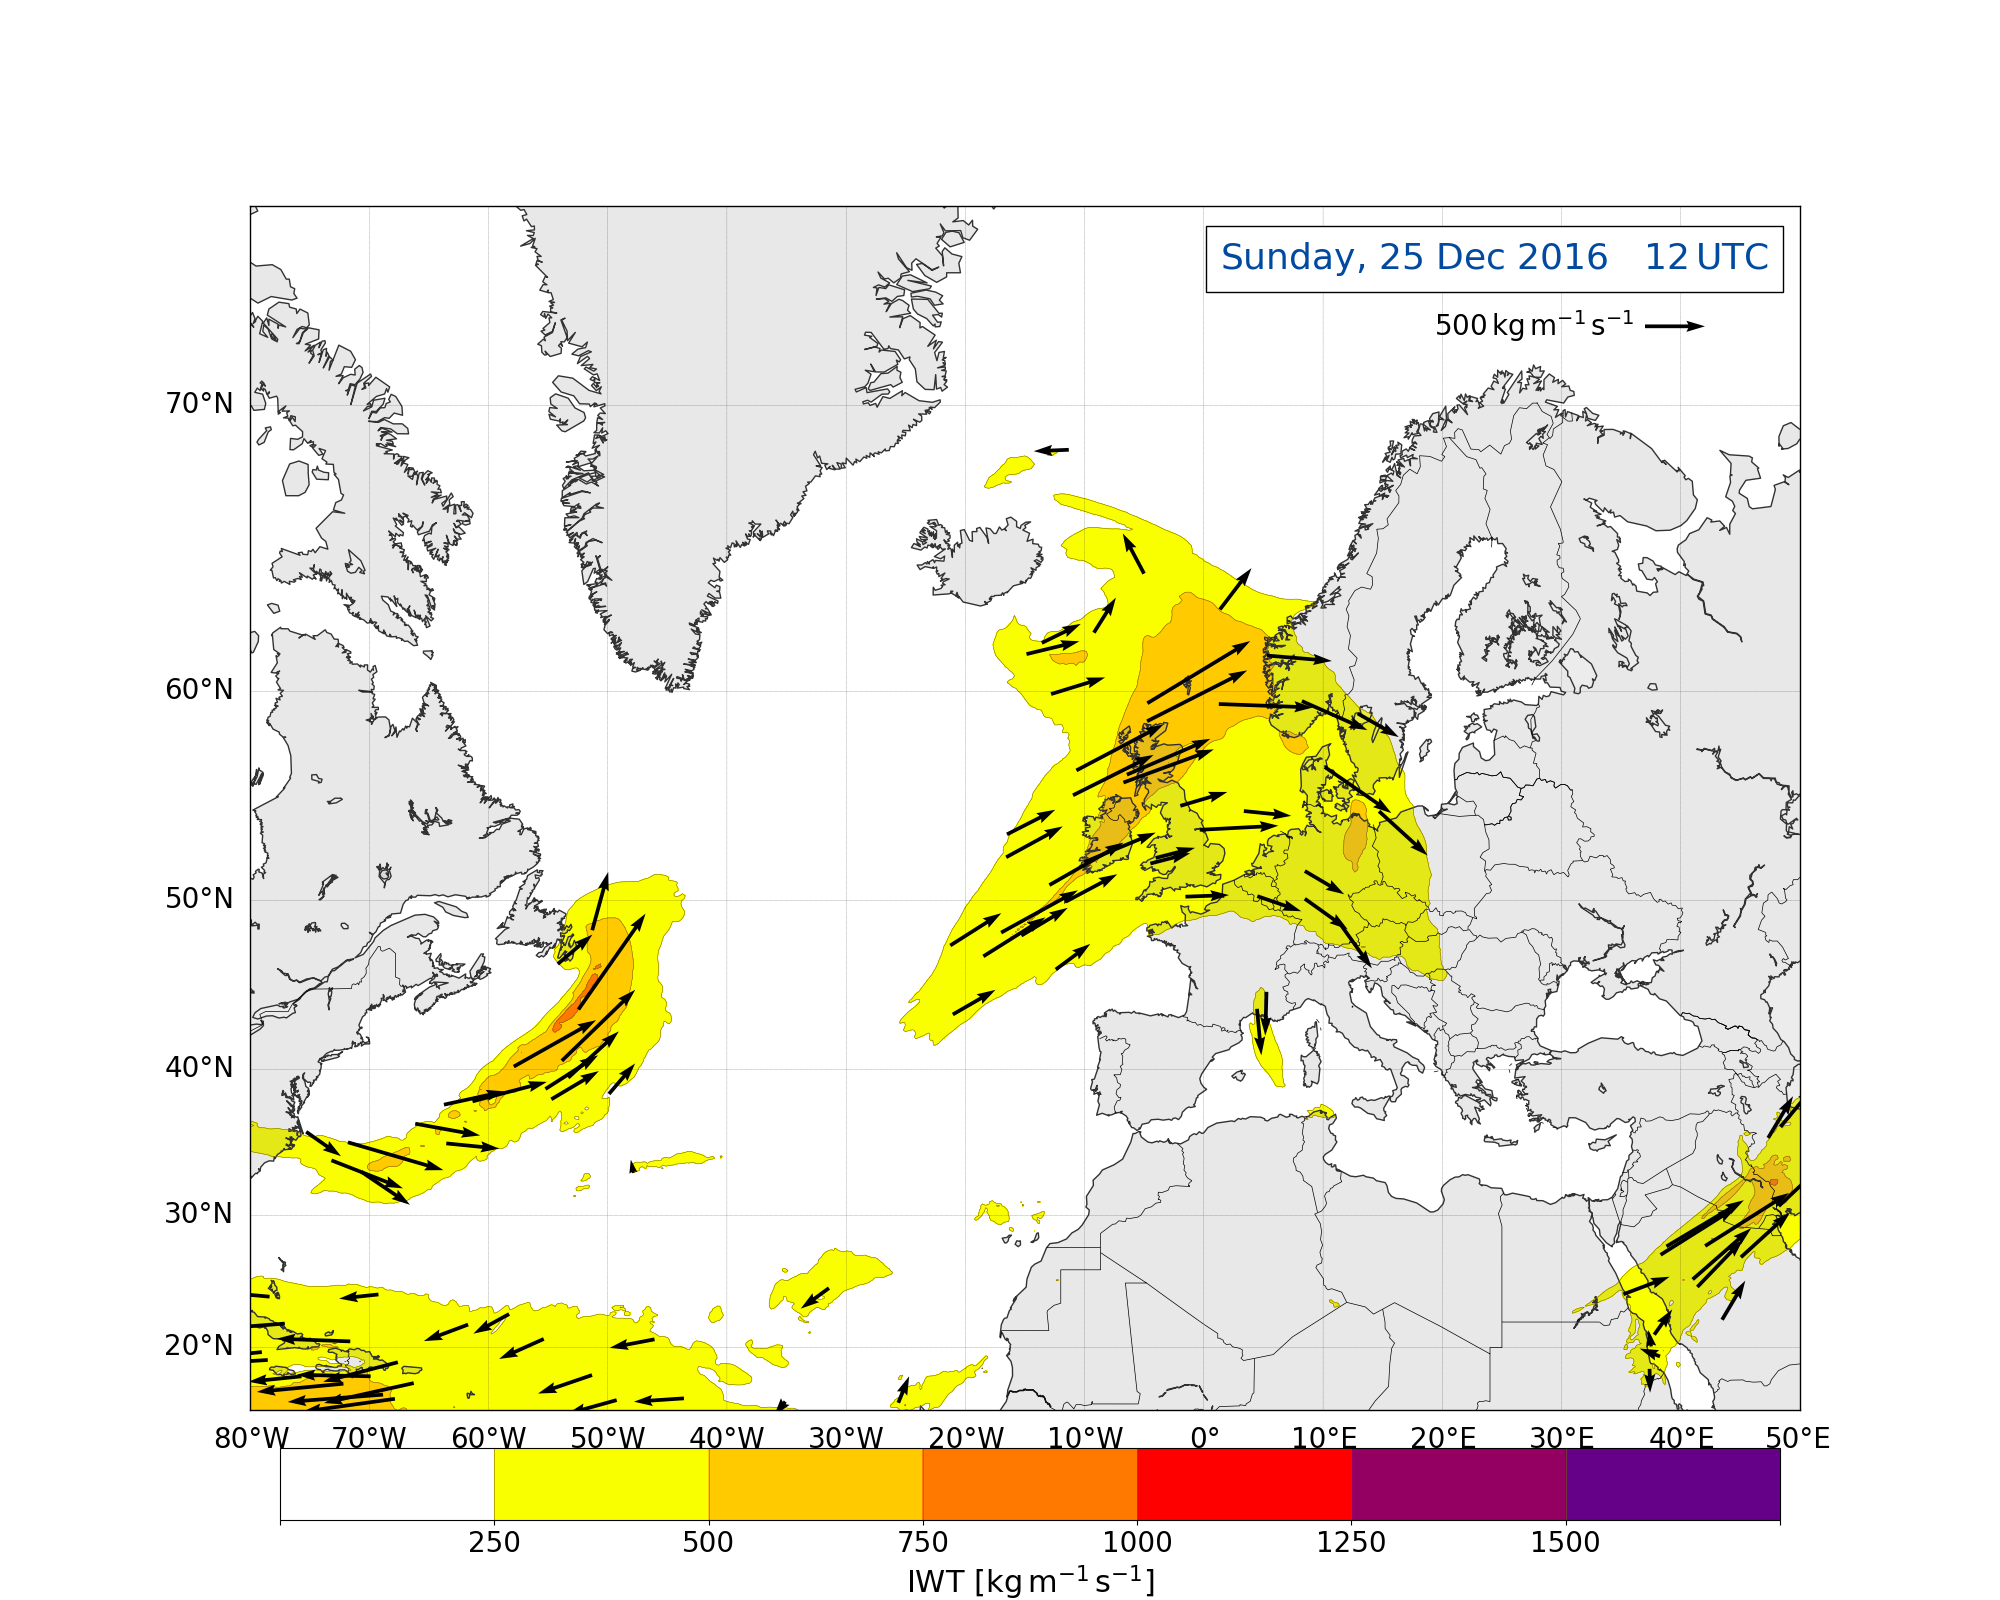
\includegraphics[trim={4.2cm 3.9cm 4.3cm 5.1cm},clip,
		width=\textwidth]{./fig_Atm_Riv/20161225_12}
		\caption{}\label{fig:AR25}
	\end{subfigure}
	%	\centering
	%%%%%% 26/12
	\begin{subfigure}[b]{0.49\textwidth}
		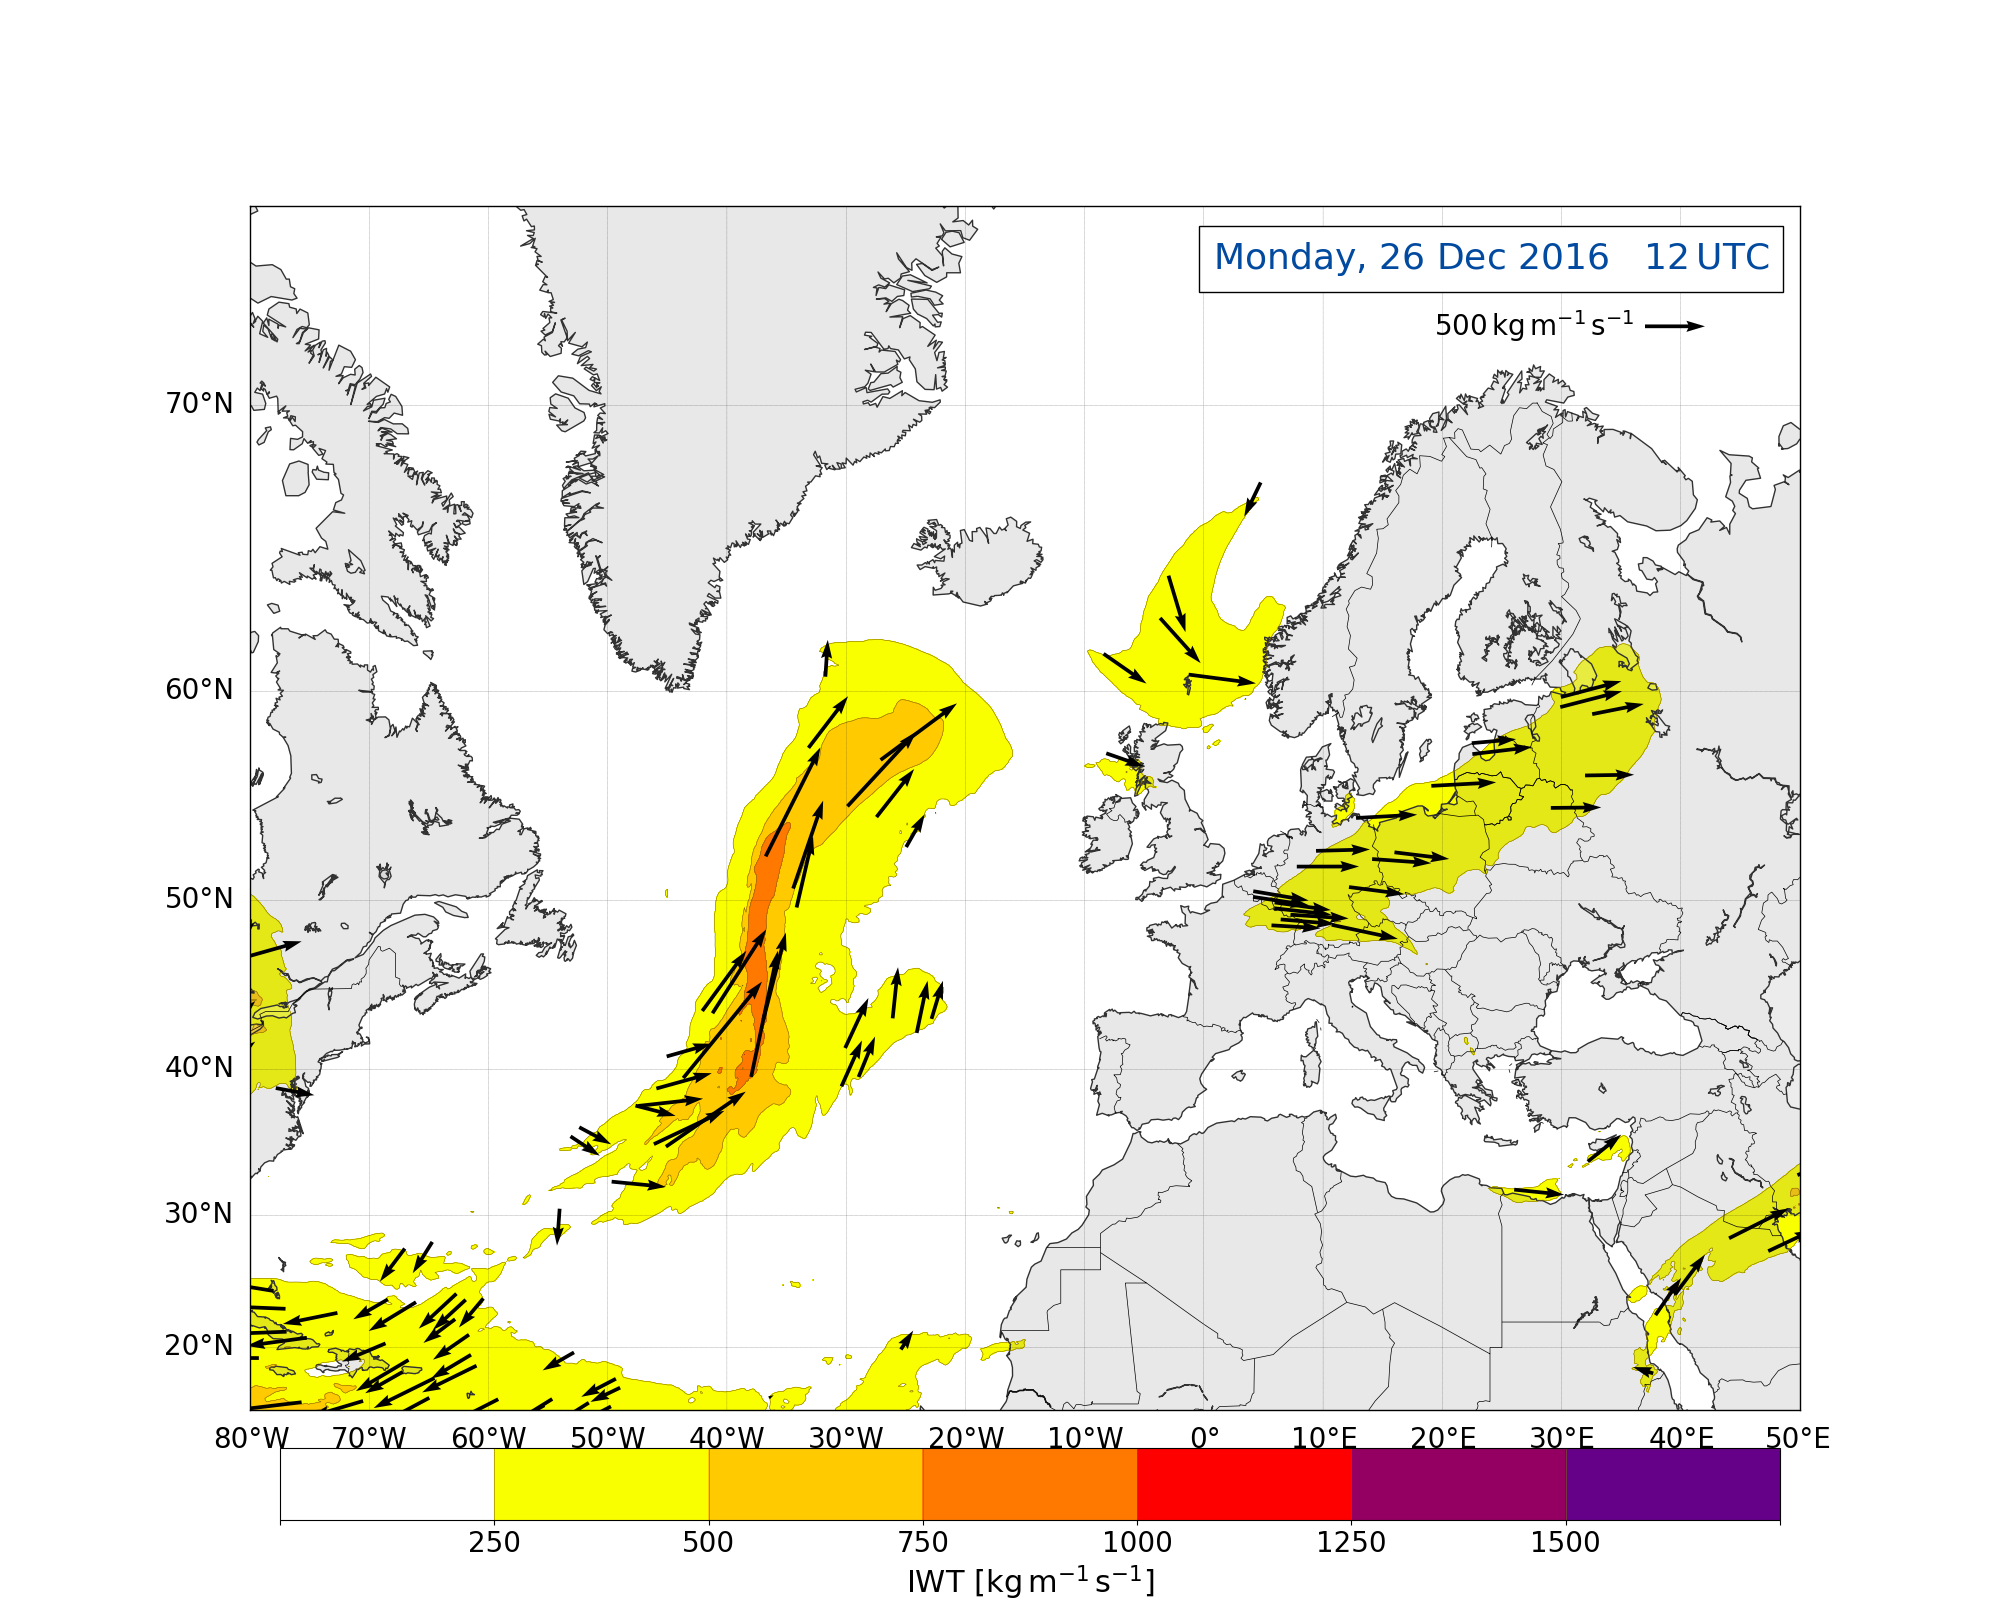
\includegraphics[trim={4.2cm 3.9cm 4.3cm 5.1cm},clip,
		width=\textwidth]{./fig_Atm_Riv/20161226_12}
		\caption{}\label{fig:AR26}
	\end{subfigure}
	%%%%%% 27/12
	\begin{subfigure}[b]{0.49\textwidth}
		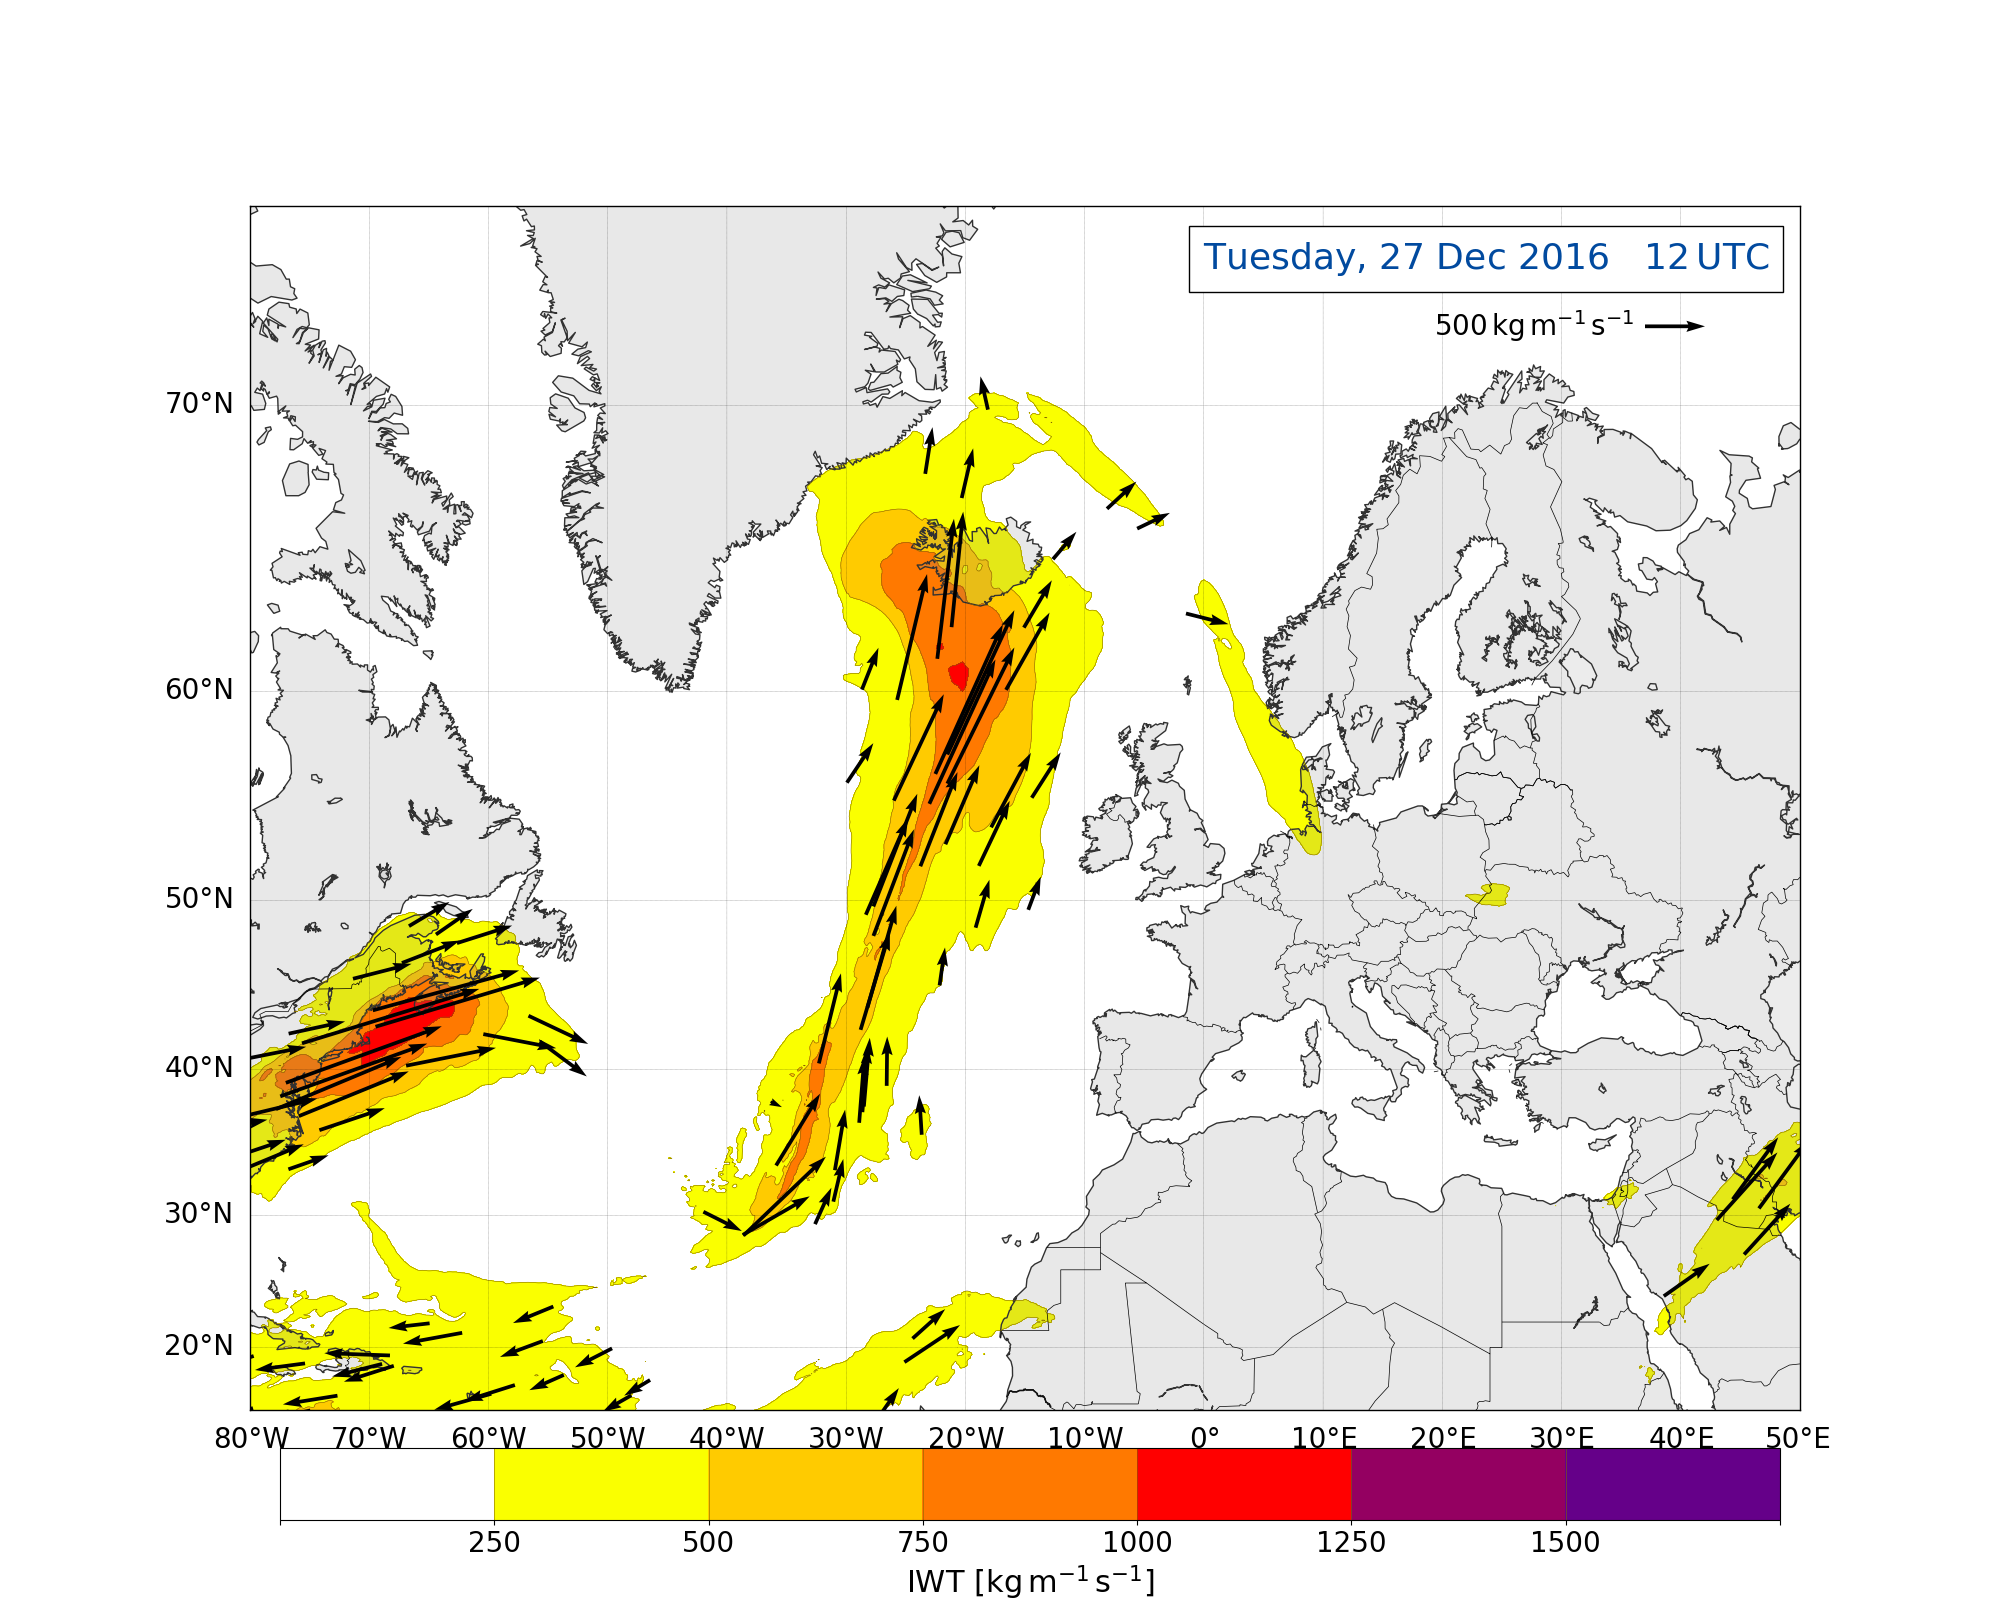
\includegraphics[trim={4.2cm 3.9cm 4.3cm 5.1cm},clip,
		width=\textwidth]{./fig_Atm_Riv/20161227_12}
		\caption{}\label{fig:AR27}
	\end{subfigure}
	%%%%%% label
	\begin{subfigure}[b]{\textwidth}
		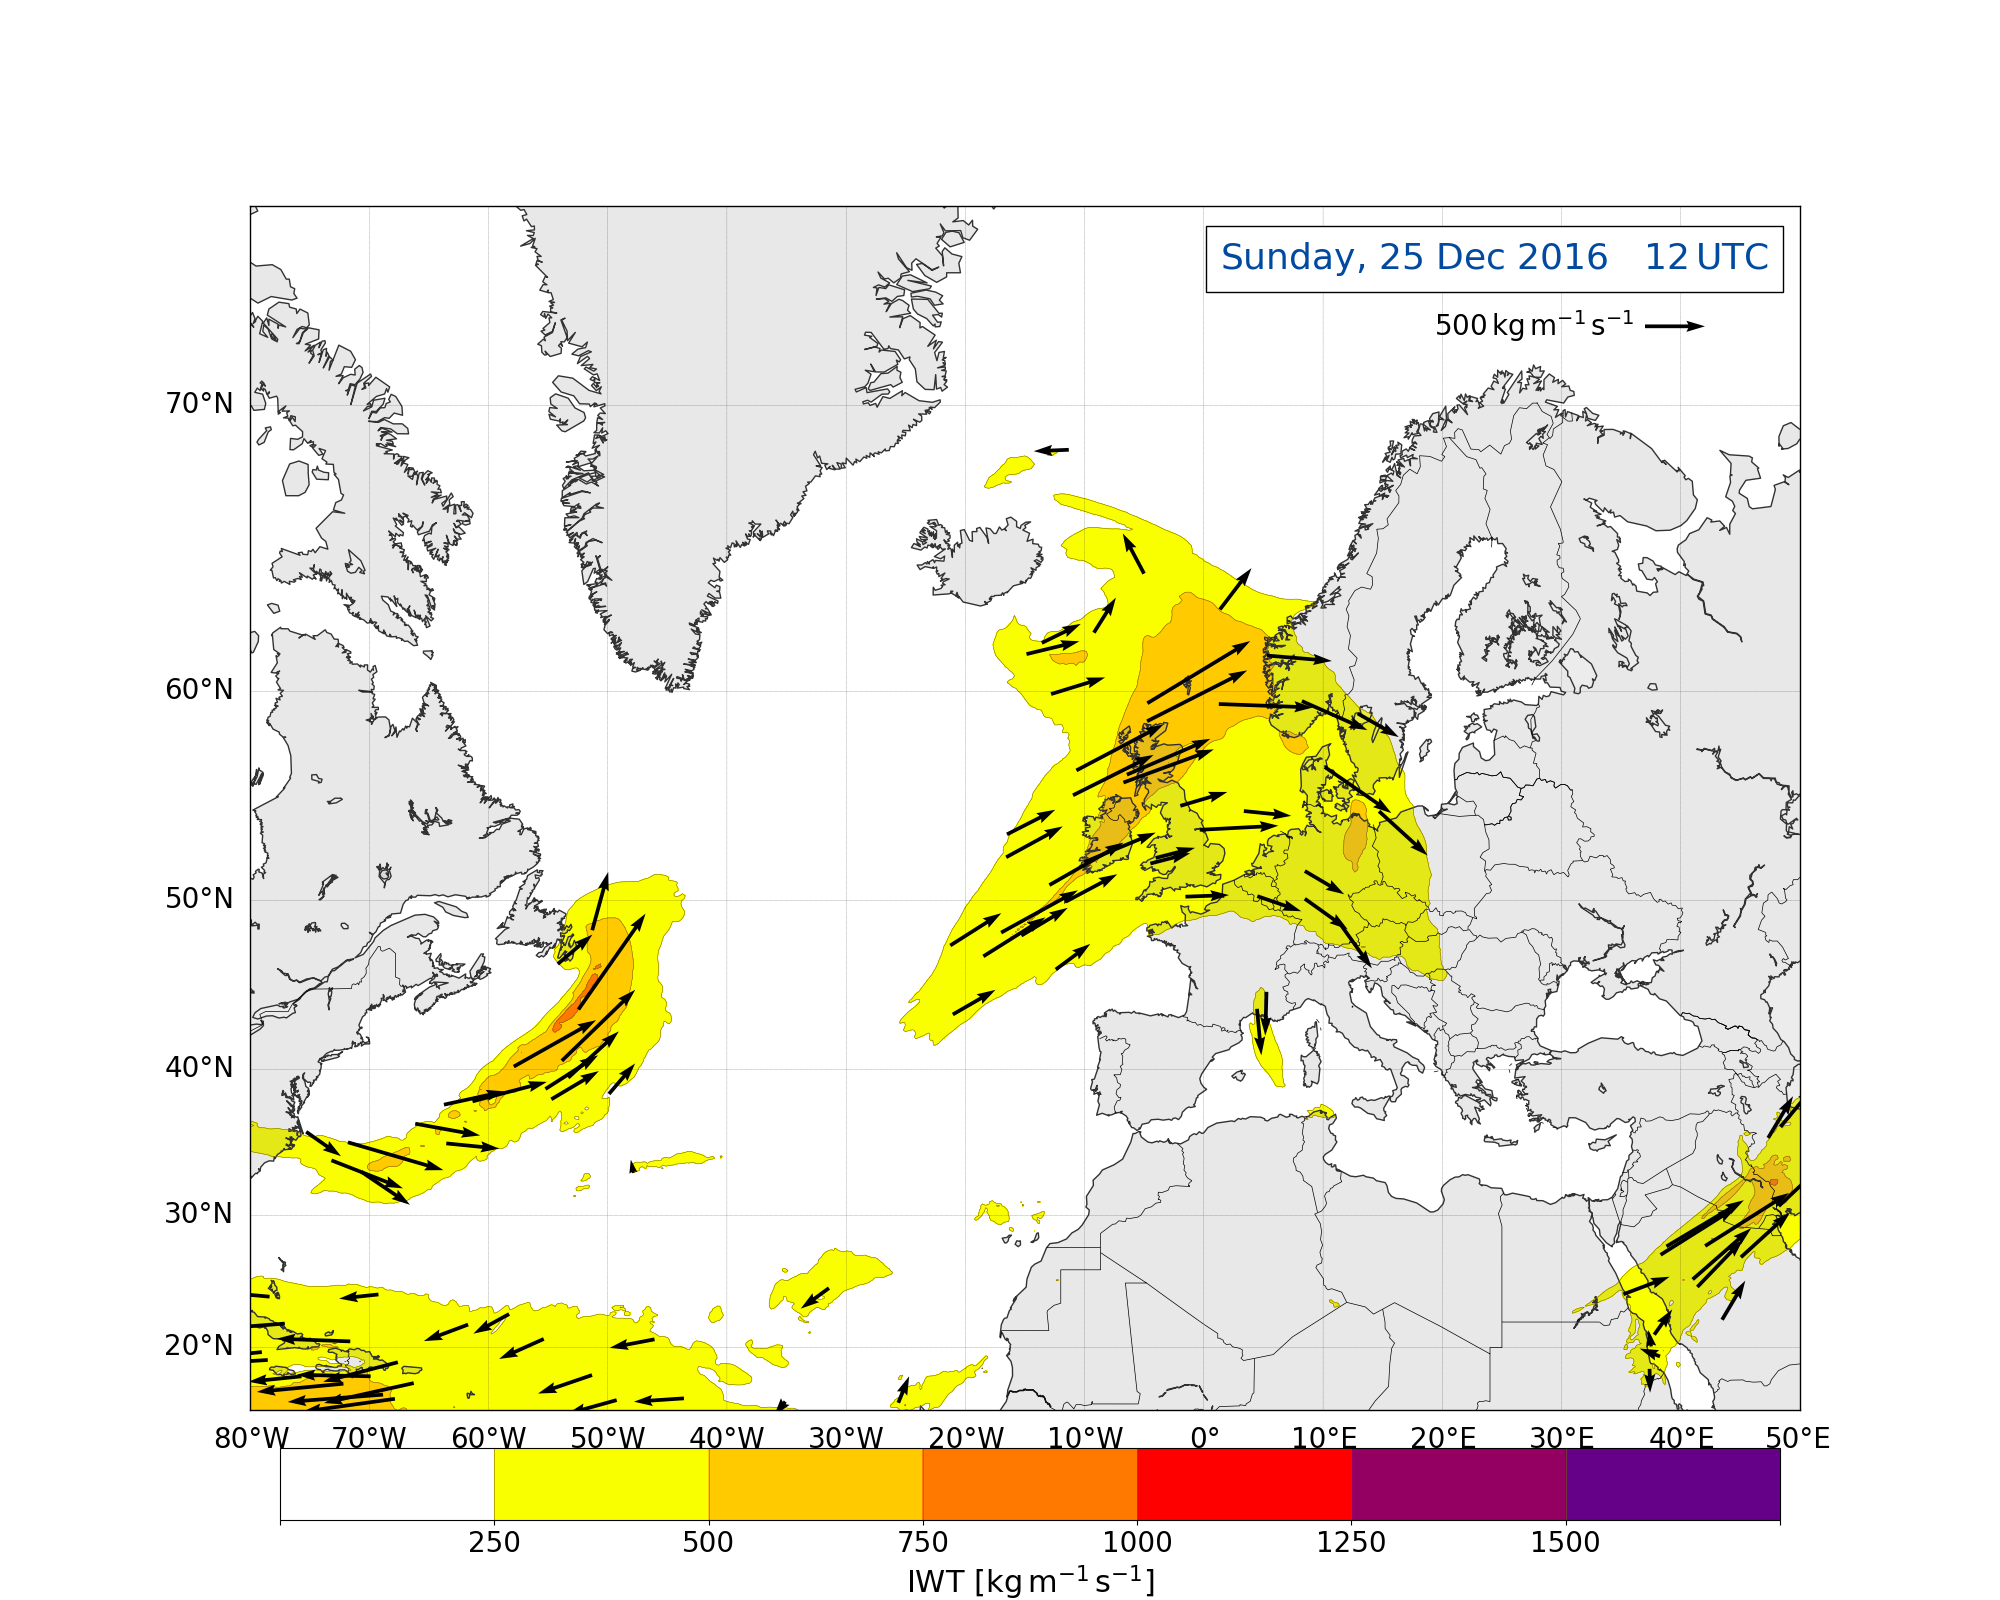
\includegraphics[trim={4.2cm 0cm 4.3cm 36.8cm},clip,
		width=\textwidth]{./fig_Atm_Riv/20161225_12}
	\end{subfigure}
    \caption{\textit{(Continued from previous page.)}}
\end{figure}
%%%%%%%%%%%%%%%%%%%%%%%%%%%%%%%%%%%%%%%%%%%%%%%%%%%%%%%%%%%%%%%%%%%%%%%%

